\documentclass[8pt, landscape, a4paper]{extarticle}

% --- 核心宏包 ---
\usepackage[UTF8]{ctex}
\usepackage[margin=0.8cm, top=1cm, bottom=1.3cm]{geometry}
\usepackage{multicol}
\usepackage{xcolor}
\usepackage{tcolorbox}
\usepackage{enumitem}
\usepackage{amsmath}
\usepackage{amssymb}
\usepackage{fontspec}
\usepackage{tikz}
\usetikzlibrary{arrows.meta, shapes}

% --- 去掉页码 ---
\pagestyle{empty}

% --- 颜色定义 (Black/Gray 主题) ---
\definecolor{headerblue}{RGB}{40, 40, 40}      % Dark Gray
\definecolor{navcolor}{RGB}{211, 84, 0}        % 导航橙
\definecolor{intuitioncolor}{RGB}{41, 128, 185}% 直觉蓝
\definecolor{accentcolor}{RGB}{192, 57, 43}    % 强调红
\definecolor{section2}{RGB}{22, 160, 133}      % 绿色
\definecolor{dividergray}{RGB}{220, 220, 220}

% --- 全局设置 ---
\setlength{\parindent}{0pt}
\setlength{\columnsep}{0.4cm} 
\linespread{1.1} 

% --- 列表样式 ---
\setlist[itemize]{leftmargin=1.2em, nosep, itemsep=2pt, topsep=2pt, label=$\textcolor{headerblue}{\vcenter{\hbox{\tiny$\bullet$}}}$ }
\setlist[description]{leftmargin=0.2em, style=sameline, nosep, itemsep=2pt, font=\bfseries}

% --- Box 样式 ---
\newtcolorbox{mybox}[2][]{%
  colback=white,
  colframe=#2,
  coltitle=white,
  boxrule=1pt,             
  arc=2mm,                 
  left=4pt, right=4pt, top=3pt, bottom=3pt, 
  toptitle=3pt, bottomtitle=3pt, 
  fonttitle=\bfseries\sffamily\large,
  title={#1},
  after skip=5pt          
}

% --- 自定义命令 ---
\newcommand{\subt}[1]{{\vspace{2pt}\textbf{\large \textcolor{black}{#1}}}}

\newcommand{\boxdesc}[1]{%
    \textit{\small \textcolor{gray}{#1}}%
    \par\vspace{2pt}%
    {\color{dividergray}\hrule height 0.5pt}%
    \vspace{2pt}%
}

\newcommand{\sepline}{%
    \par \vspace{3pt}%
    {\color{dividergray}\hrule height 0.5pt}%
    \par \vspace{3pt}%
}

% 公式间距
\setlength{\abovedisplayskip}{3pt}
\setlength{\belowdisplayskip}{3pt}

\begin{document}

% --- 页眉 ---
\begin{center}
    {\Huge \textbf{\sffamily \textcolor{headerblue}{张量分析 Tensor Calculus Cheat Sheet}}} \\
    \vspace{0.2cm}
    {\large \texttt{The Language of Physics: Invariance and Covariance}}
\end{center}

% --- 开始四栏布局 ---
\begin{multicols*}{4}

% === 第一栏 ===

\begin{mybox}[️ 场景导航 (Use Cases)]{navcolor}
    \boxdesc{遇到什么问题 $\to$ 用什么工具}
    \begin{itemize}[itemsep=2pt]
        \item \textbf{广义相对论} $\to$ 黎曼曲率张量 / 爱因斯坦方程
        \item \textbf{流体力学} $\to$ 应力张量 / 纳维-斯托克斯
        \item \textbf{深度学习} $\to$ 多维数组运算 (PyTorch)
        \item \textbf{连续介质力学} $\to$ 应变张量
        \item \textbf{电磁学} $\to$ 麦克斯韦张量 $F_{\mu\nu}$
        \item \textbf{微分几何} $\to$ 形式与向量场
    \end{itemize}
\end{mybox}

\begin{mybox}[1. 基础定义 (Foundations)]{headerblue}
    \boxdesc{坐标变换的规律}
    
    \subt{爱因斯坦求和约定}
    上下指标重复即求和。
    $$ v^i e_i = \sum_{i=1}^n v^i e_i $$
    \sepline
    
    \subt{逆变向量 (Contravariant) $v^i$}
    像坐标微分 $dx^i$ 一样变换 (上标)。
    $$ \bar{v}^i = \frac{\partial \bar{x}^i}{\partial x^j} v^j $$
    \sepline
    
    \subt{协变向量 (Covariant) $u_i$}
    像梯度 $\frac{\partial \phi}{\partial x^i}$ 一样变换 (下标)。
    $$ \bar{u}_i = \frac{\partial x^j}{\partial \bar{x}^i} u_j $$
    \textit{直觉: 逆变是箭头,协变是等高线。}
\end{mybox}

\begin{mybox}[2. 度量张量 (Metric Tensor)]{headerblue}
    \boxdesc{升降指标的梯子}
    
    \subt{定义 $g_{ij}$}
    $$ ds^2 = g_{ij} dx^i dx^j $$
    \begin{itemize}
        \item \textbf{降指标}: $v_i = g_{ij} v^j$。
        \item \textbf{升指标}: $v^i = g^{ij} v_j$ ($g^{ij}$ 是 $g_{ij}$ 的逆矩阵)。
    \end{itemize}
    \sepline
    
    \subt{内积}
    $$ \mathbf{u} \cdot \mathbf{v} = g_{ij} u^i v^j = u^i v_i $$
\end{mybox}

\columnbreak

% === 第二栏 ===

\begin{mybox}[3. 协变导数 (Covariant Derivative)]{headerblue}
    \boxdesc{弯曲空间怎么求导?}
    
    \subt{问题}
    普通偏导 $\partial_i v^j$ 不是张量 (因为基底也在变)。
    \sepline
    
    \subt{定义 $\nabla_i v^j$}
    $$ \nabla_i v^j = \partial_i v^j + \Gamma^j_{ik} v^k $$
    \begin{itemize}
        \item $\Gamma^j_{ik}$: \textbf{克里斯托费尔符号} (Christoffel Symbols)。
        \item 修正项描述了坐标系的弯曲/扭曲。
    \end{itemize}
    \sepline
    
    \subt{对于标量}
    $\nabla_i \phi = \partial_i \phi$ (标量没有方向,无需修正)。
\end{mybox}

\begin{mybox}[4. 曲率 (Curvature)]{headerblue}
    \boxdesc{平移一圈回不到原点}
    
    \subt{黎曼曲率张量 $R^\rho_{\sigma\mu\nu}$}
    $$ [\nabla_\mu, \nabla_\nu] v^\rho = R^\rho_{\sigma\mu\nu} v^\sigma $$
    衡量协变导数的不可交换性。
    \sepline
    
    \subt{里奇张量 (Ricci) $R_{\mu\nu}$}
    $R_{\mu\nu} = R^\lambda_{\mu\lambda\nu}$ (缩并)。
    \textbf{里奇标量 $R$}: $R = g^{\mu\nu} R_{\mu\nu}$。
    \textit{物理意义: 描述体积的扭曲。}
\end{mybox}

\columnbreak

% === 第三栏 ===

\begin{mybox}[5. 物理应用 (Physics)]{headerblue}
    \boxdesc{宇宙的方程}
    
    \subt{爱因斯坦场方程 (GR)}
    $$ R_{\mu\nu} - \frac{1}{2}R g_{\mu\nu} = \frac{8\pi G}{c^4} T_{\mu\nu} $$
    \textit{几何 (左边) = 物质 (右边)。时空告诉物质如何运动,物质告诉时空如何弯曲。}
    \sepline
    
    \subt{麦克斯韦方程组}
    $$ \partial_\mu F^{\mu\nu} = \mu_0 J^\nu $$
    $F^{\mu\nu}$ 是电磁场张量。四个方程合而为一。
\end{mybox}

\begin{mybox}[6. 常用算子 (Operators)]{headerblue}
    \boxdesc{梯度、散度、旋度}
    
    \subt{梯度 (Gradient)}
    $(\nabla f)^i = g^{ij} \partial_j f$
    \sepline
    
    \subt{散度 (Divergence)}
    $\nabla \cdot v = \nabla_i v^i = \frac{1}{\sqrt{g}} \partial_i (\sqrt{g} v^i)$
    \sepline
    
    \subt{拉普拉斯 (Laplacian)}
    $\Delta f = \nabla_i \nabla^i f = \frac{1}{\sqrt{g}} \partial_i (\sqrt{g} g^{ij} \partial_j f)$
\end{mybox}

\begin{mybox}[7. Python / EinsteinPy 实战]{headerblue}
    \boxdesc{代码工具箱}
    \begin{itemize}
        \item \textbf{Einstein Summation}:
        \texttt{np.einsum('ij,jk->ik', A, B)} (矩阵乘法)
        \texttt{np.einsum('ii', A)} (迹)
        \item \textbf{EinsteinPy}: 广义相对论库。
        \item \textbf{SymPy.diffgeom}: 符号计算张量。
    \end{itemize}
\end{mybox}

\columnbreak

% === 第四栏 ===

\begin{mybox}[8. 高阶前沿 (Advanced)]{headerblue}
    \boxdesc{超越张量}
    
    \subt{旋量 (Spinor)}
    “半个”向量。旋转 360 度变号,旋转 720 度才复原。
    \textit{描述电子等费米子。}
    \sepline
    
    \subt{李导数 (Lie Derivative) $\mathcal{L}_X$}
    不需要度量,只需要流形结构。
    描述张量场沿流线的变化。
    \sepline
    
    \subt{外微分形式 (Forms)}
    反对称的张量。
    $d, \wedge, *$ (Hodge Star)。
    \textit{比指标记法更优雅、更几何。}
\end{mybox}

\vspace*{\fill}

\begin{mybox}[ 核心直觉 (Intuition)]{intuitioncolor}
    \boxdesc{“物理定律对坐标系免疫。”}
    
    % TikZ 矢量图: 协变与逆变基底
    \begin{center}
    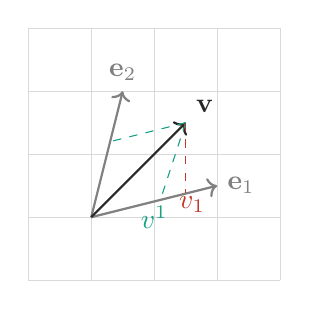
\begin{tikzpicture}[scale=0.8]
        % 坐标网格 (斜的)
        \draw[gray!30] (-1,-1) grid (3,3); % 假装是直角
        \draw[->, thick, gray] (0,0) -- (2, 0.5) node[right] {$\mathbf{e}_1$};
        \draw[->, thick, gray] (0,0) -- (0.5, 2) node[above] {$\mathbf{e}_2$};
        
        % 向量 v
        \draw[->, thick, headerblue] (0,0) -- (1.5, 1.5) node[above right] {$\mathbf{v}$};
        
        % 逆变分量 (平行投影)
        \draw[dashed, section2] (1.5, 1.5) -- (1.1, 0.28); % 平行于 e2
        \draw[dashed, section2] (1.5, 1.5) -- (0.3, 1.2); % 平行于 e1
        \node[section2] at (1, 0) {$v^1$};
        
        % 协变分量 (垂直投影)
        \draw[dashed, accentcolor] (1.5, 1.5) -- (1.5, 0.38); % 垂直于 e1
        \node[accentcolor] at (1.6, 0.2) {$v_1$};
        
    \end{tikzpicture}
    \end{center}

    \hspace{1em}张量不仅仅是多维数组,它是\textbf{几何实体}。
    \vspace{4pt}
    
    \subt{三大核心视角}
    \begin{itemize}[itemsep=4pt]
        \item \textbf{坐标无关性}: 
        张量方程 (如 $T_{\mu\nu} = 0$) 在一个坐标系下成立,则在所有坐标系下成立。这是广义相对论的基石 (广义协变性原理)。
        
        \item \textbf{指标体操}: 
        上标和下标的缩并 (Contraction) 本质上是矩阵乘法或求迹。学会熟练地升降指标,你就能在弯曲时空中自由穿梭。
        
        \item \textbf{几何修正}: 
        $\Gamma$ (联络) 不是张量,它是坐标系弯曲产生的“惯性力” (如离心力、科里奥利力)。把它加上去,导数就变成了真正的几何导数 (协变导数)。
    \end{itemize}
    
    \vspace{6pt}
    \centering\textit{\footnotesize 无论你怎么扭曲时空,张量依然是张量。}
\end{mybox}

\end{multicols*}

\end{document}
